\chapter{Problemy i ich rozwiązania}
\label{problems_and_solutions}

Nieodłączną częścią każdego projektu informatycznego i elektronicznego są problemy związane z uruchomieniem. Nie inaczej było w przypadku niniejszej pracy i opisywanego w nim systemu. W trakcie jego rozwoju napotkano szereg różnorakich komplikacji, z którymi należało sobie poradzić. W tym rozdziale dokonano wyboru i krótkiego opisu wraz z solucją trzech najciekawszych z nich.


\section{Zawieszanie urządzenia lokalizującego}

Pierwszy z wybranych problemów dotyczył pierwszych momentów uruchomienia lokalizatora. Polegał on na tym, że mimo poprawnego zaprogramowania mikrokontrolera i działającej poprawnie apkilacji z podłączonym do niej debuggerem, po jego odłączeniu i dokonaniu resetu urządzenia urządzenie zawieszało się gdzieś we wstępnej fazie inicjalizacji. Można to było wywnioskować po fakcie, iż zapalała się dioda LED, sterowana programowo, lecz moduł GSM nigdy nie rozpoczynał swej inicjalizacji. Po wczytaniu się w notę katalogową producenta mikrokontrolera okazało się, iż problem stanowił wykorzystywany do odmierzania czasu, wbudowany w rdzeń przez firmę ARM zegar systemowy SysTick. Powodem jego błędnej pracy było każdorazowe wejście mikrokontrolera w tryb oszczędzania energii w trakcie oczekiwania na upłynięcie określonej ilości czasu (\textit{ang. delay}). Powoduje on bowiem zatrzymanie sygnału taktującego rdzeń mikrokontrolera, a tym samym - SysTick'a, wykorzystującego zegar systemowy. Efektem jest wówczas praca w pętli i oczekiwanie na upłynięcie losowej ilości czasu. Losowość ta jest wywołana faktem, iż rdzeń wybudzany jest dowolnym przerwaniem na pewien krótki czas, a zatem SysTick "ożywał" na krótko by znów ulec po chwili zatrzymaniu. Co ciekawe, problem ten nie występował w trakcie pracy z debuggerem, ponieważ wymusza on ciągłą pracę zegara systemowego niezależnie od trybu oszczędzania energii. 

Rozwiązaniem było zastąpienie SysTick'a innym zegarem - wbudowanym w mikrokontroler bardzo energooszczędnym zegarem RTC (\textit{ang. \textbf{R}eal \textbf{T}ime \textbf{C}lock}).

\section{Brak danych z GPS}

Kolejny problem związany był typowo z elektroniką. Polegał on na tym, że mimo włączania modułu GPS zgodnie z notą katalogową producenta chip'a GSM i GPS - poprzez komendę AT wysyłaną poprzez interfejs UART do pośredniczącego modułu GSM, moduł GPS nie odpowiadał. Ponadto, nie był responsywny na żadną inną komendę. Problem ten wynikał z błędnego zrozumienia noty katalogowej od producenta, dotyczącej zasilania modułu GPS. Posiada on bowiem osobny pin, do którego powinno zostać dostarczone zasilanie (\textit{GNSS\_VCC}) oraz pin (\textit{GNSS\_VCC\_EN}), który przyjmuje stan wysoki (napięcie o wartości ok. 3.3 V) gdy GPS jest włączony oraz stan niski (napięcie bliskie 0 V) gdy jest wyłączony. Pin \textit{GNSS\_VCC\_EN} reagował poprawnie - zmieniał stan po włączeniu modułu GPS komendą AT. Błędnym rozumowaniem okazało się założenie, że jest to jedynie fizyczny wskaźnik statusu zasilania modułu GPS. W praktyce, zamysłem producenta chip'a było, aby pin ten wysterowywał tranzystor bądź zewnętrzne źródło zasilania, w celu podania napięcia na pin \textit{GNSS\_VCC}. Wynika to z faktu występowania sztywnych zależności czasowych w wewnętrznej komunikacji między modułami GSM i GPS. Rozwiązaniem tego problemu było przeprojektowanie zasilania modułu GPS zgodnie z założeniem producenta chip'a. Przedstawiono to na rysunku \ref{fig:image_mistake_gps_power}.

\begin{figure}[H]
\centering
	\subfloat[Błędny schemat zasilania modułu GPS.]
	{
	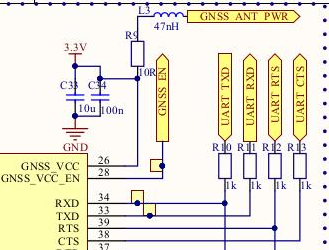
\includegraphics[width=7cm]{img/Problems/gps_power_old.png}
	}
	\qquad
	\subfloat[Poprawiony schemat zasilania modułu GPS.]
	{
	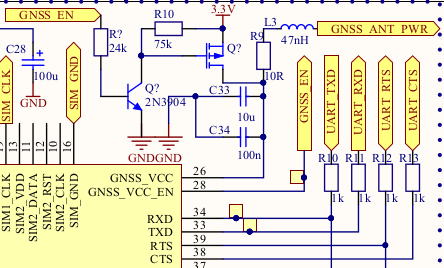
\includegraphics[width=7cm]{img/Problems/gps_power_new.png}
	}
	
	\caption{Schematy zasilania modułu GPS. Źródło: Twórczość własna}
	\label{fig:image_mistake_gps_power}
\end{figure}

\section{Kompensacja wpływu przyspieszenia ziemskiego}

Występowanie przyspieszenia ziemskiego w systemach pomiaru przyspieszeń bywa często uciążliwe. Problem ten występowałby jedynie dla jednej osi, gdyby urządzenia były idealnie zorientowane względem Ziemi, czyli oś Z akcelerometru pokrywałaby się z kierunkiem działania siły grawitacji. Ponieważ jest to praktycznie niemożliwe do osiągnięcia, zwłaszcza w pojazdach, wartość przyspieszenia ziemskiego będzie rzutowana nie tylko na oś Z, ale także X i Y. Jest to działanie niepożądane, ponieważ stanowi stały składnik dodawany do mierzonych przyspieszeń (\textit{ang. offset}), co zaburza pomiar. W związku z tym, na etapie inicjalizacji urządzenia lokalizującego należy dokonać pomiaru przyspieszeń we wszystkich osiach (przy założeniu bezruchu urządzenia), a następnie od każdej próbki przyspieszenia odejmować te wartości.
Pierwotnie w tym celu wykorzystywano funkcjonalność wbudowaną w moduł akcelerometru. Producent wbudował w niego bowiem rejestry, których zawartości odejmowane są sprzętowo od wyników pomiaru. Rozwiązanie to brzmi idealnie, ponieważ ze względu na wykonaniu tej operacji przez akcelerometr nie zwiększałaby ilości operacji niezbędnych do wykonania przez mikrokontroler. Niestety problemem okazała się rozdzielczość tychże rejestrów. Posiadają one pojemność 8 bitów ze znakiem (wartości od -128 do 127) i programowalną rozdzielczość w dwustopniowym zakresie. Do wyboru są dwie wartości: $2^{-6}g/LSB$ (\textit{ang. \textbf{L}east \textbf{S}ignificant \textbf{B}it}) lub $2^{-10}g/LSB$. 
Po krótkich obliczeniach okazało się, że ta druga wartość nie pozwoli na pełną likwidację wartości przyspieszenia ziemskiego, ponieważ:

\begin{equation}
A_{max} = 2^{-10} \cdot 9.81\frac{m}{s^2} \cdot 127 \approx 1.216 \frac{m}{s^2}
\end{equation}

Gdzie $A_{max}$ wskazuje maksymalną wartość, która może zostać skompensowana. Jak widać, w przypadku tej rozdzielczości nie jest ona dostatecznie duża. Pozostaje więc jedynie wybór $2^{-6} g$:

\begin{equation}
A_{max} = 2^{-6} \cdot 9.81\frac{m}{s^2} \cdot 127 \approx 19.467 \frac{m}{s^2}
\end{equation}

Jak widać, przy tej rozdzielczości można teoretycznie bezproblemowo usunąć wpływ grawitacji. Jednakże w tym przypadku pojawia się inny kłopot - rozdzielczości pojedynczego bitu:

\begin{equation}
A_{min} = 2^{-6} \cdot 9.81\frac{m}{s^2} \approx 0.153 \frac{m}{s^2}
\end{equation}

gdzie $A_{min}$ jest wartością przyspieszenia kompensowaną przez pojedynczą jednostkę w wartości rejestru. Jak widać, maksymalny błędny wynik pomiaru, pomimo kompensacji wpływu grawitacji wynosi około $0.152(9) \frac{m}{s^2}$, co w przypadku analizy stylu jazdy wprowadza już znaczny błąd. 

Z tego powodu postanowiono zrezygnować z wykorzystania sprzętowej kompensacji i zastosować programową. W tym celu, w trakcie inicjalizacji urządzenia przez sekundę zbierane są próbki przyspieszenia, przy założeniu bezruchu pojazdu. Ich wartości w osiach X, Y i Z są uśredniane, a następnie odejmowane od każdej zebranej próbki w przyszłości. Dzięki temu, zmierzony doświadczalnie błąd kompensacji wynosił maksymalnie:

 \begin{equation}
A_{min} = 5 \cdot 19.62\frac{m}{s^2}/2^15 \approx 0.003 \frac{m}{s^2}
\end{equation}

Wynik ten jest dwa rzędy wielkości lepszy niż przy sprzętowej kompensacji.